\documentclass[crop,tikz]{standalone}% 'crop' is the default for v1.0, before it was 'preview'
\usepackage{tikz,calc,pgfplots}
\usepackage{tikz-3dplot}
\usetikzlibrary{calc}
\usetikzlibrary{calc,patterns,decorations.pathmorphing,decorations.markings}
\usetikzlibrary{shapes.geometric}
\begin{document}


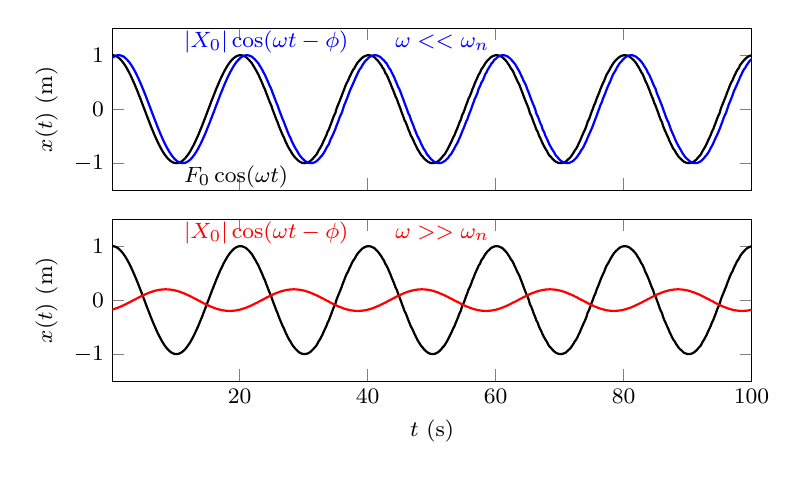
\begin{tikzpicture}[scale=1]
	\footnotesize
\begin{axis}[
	at={(0,0.2\textwidth)},
	width=0.8\textwidth,
	height=0.3\textwidth,
	ylabel = {$x(t)$ (m)},
	xticklabel=\empty,
	xmax=100,
	xmin=0.1,
	ymax=1.5,
	ymin=-1.5,
	samples=500]
	
	\def\wn{50*2*pi};
	\def\PHI{-pi/10};
	
	\addplot[black, thick, domain=0.1:100] (x, {1*cos(deg(\wn * x))});
	\addplot[blue, thick, domain=0.1:100] (x, {1 * cos(deg(\wn * x + \PHI))});		
	\node at (axis cs: 10, 1.25)  [blue, anchor=west]  {$|X_0| \cos(\omega t -\phi) \quad \quad \omega<<\omega_n$};
	\node at (axis cs: 10, -1.25)  [black, anchor=west]  {$F_0 \cos(\omega t)$};
\end{axis}


\begin{axis}[
	at={(0,0.\textwidth)},
	width=0.8\textwidth,
	height=0.3\textwidth,
	xlabel={$t$ (s)},
	ylabel = {$x(t)$ (m)},
	xmax=100,
	xmin=0.1,
	ymax=1.5,
	ymin=-1.5,
	samples=500]
	
	\def\wn{50*2*pi};
	\def\PHI{pi/1.2};
	
	\addplot[black, thick, domain=0.1:100] (x, {1*cos(deg(\wn * x))});
	\addplot[red, thick, domain=0.1:100] (x, {0.2 * cos(deg(\wn * x - \PHI))});		
	\node at (axis cs: 10, 1.25)  [red, anchor=west]   {$|X_0| \cos(\omega t -\phi)\quad \quad \omega>>\omega_n$};
	
\end{axis}

	
\end{tikzpicture}

\end{document}